%==============================================================================
% Sjabloon poster bachproef
%==============================================================================
% Gebaseerd op document class `a0poster' door Gerlinde Kettl en Matthias Weiser
% Aangepast voor gebruik aan HOGENT door Jens Buysse en Bert Van Vreckem

\documentclass[a0,portrait]{hogent-poster}

% Info over de opleiding
\course{Bachelorproef}
\studyprogramme{toegepaste informatica}
\academicyear{2023-2024}
\institution{Hogeschool Gent, Valentin Vaerwyckweg 1, 9000 Gent}

% Info over de bachelorproef
\title{Gepersonaliseerde route-app voor loop-
fanaten op basis van diverse online tools}
% \subtitle{Ondertitel (eventueel)}
\author{Laurens De Maeyer}
\email{laurens.demaeyer@student.hogent.be}
\supervisor{Giselle Vercauteren (Hogeschool Gent)}
\cosupervisor{Manu De Buck (We-are)}

% Indien ingevuld, wordt deze informatie toegevoegd aan het einde van de
% abstract. Zet in commentaar als je dit niet wilt.
\specialisation{Mobile and Enterprise Development}
\keywords{API, Node.js, React Native, Loopfanaten, Routeapp}
\projectrepo{https://github.com/LaurensDM/Bachelor-Thesis}

\begin{document}

\maketitle

\begin{abstract}

Deze bachelorproef concentreert zich op het onderzoek naar en de ontwikkeling van een kosteloze route-applicatie voor loopfanaten. 
Het hoofddoel is om diverse online tools, met name gratis publieke API's, te verzamelen en te integreren in deze applicatie. 
Dit om looproutes te genereren op basis van verschillende parameters zoals afstand, hoogtemeters, en ondergrond.
\end{abstract}

\begin{multicols}{2} % This is how many columns your poster will be broken into, a portrait poster is generally split into 2 columns

\section{Introductie}
In de moderne wereld,
waarin tech\-no\-lo\-gie \@ steeds belangrijker wordt,
is het niet meer dan normaal dat er ook technologie bestaat voor sporters.
Zo zijn er al verschillende apps beschikbaar voor lopers, zoals Strava, Runkeeper en Nike Run Club.
De functies dat deze apps aanbieden zijn echter niet altijd gefocust op het genereren van routes of zijn niet toegankelijk via de gratis versie van de app.
In sommige gevallen moet er een abonnement worden afgesloten om gebruik te kunnen maken van alle functies. Een API, oftewel een interface, maakt communicatie tussen verschillende applicaties mogelijk.
Welke publieke, en gratis, API's zijn er beschikbaar om routes te genereren? Welke combinatie van deze API's is het meest geschikt voor het genereren van routes voor loopfanaten? Welke functies bieden populaire route-apps aan? Welke parameters willen loopfanaten aan een route koppelen? Dit zijn de vragen die in dit onderzoek beantwoord zullen worden.

Dit onderzoek concentreert zich op het verzamelen van diverse online tools voor het genereren van een route, in de vorm van gratis open API's, 
met als doel ze te integreren in een kosteloze route-app voor loopfanaten.
Om dit te realiseren zal er een proof of concept ontwikkeld worden die gebruik maakt van de gekozen API's. 
De applicatie zal ontwikkeld worden in React Native en Node.js. React Native is een framework 
dat het mogelijk maakt om native apps te ontwikkelen voor Android en iOS\@. 
Node.js is een JavaScript runtime die het mogelijk maakt om JavaScript code te schrijven buiten de browser.
Deze proof of concept zal beschikbaar zijn op zowel Android- als iOS-systemen. Weinig zaken zijn effectief gratis, 
daarom zal er ook een kostenanalyse uitgevoerd worden om de haalbaarheid van de lancering en het onderhoud van de applicatie te beoordelen.

\section{Experimenten}

A newt? Camelot! Why? No, no, no! Yes, yes. A bit. But she's got a wart.
Shut up! I dunno. Must be a king. Who's that then? Look, my liege! On second thoughts, let's not go there. It is a silly place.
Shut up! Will you shut up?! No, no, no! Yes, yes. A bit. But she's got a wart. He hasn't got shit all over him. It's only a model. It's only a model.
Bring her forward! I don't want to talk to you no more, you empty-headed animal food trough water! I fart in your general direction! Your mother was a hamster and your father smelt of elderberries! Now leave 

\section{Sectie met figuur}


\begin{center}
  \captionsetup{type=figure}
  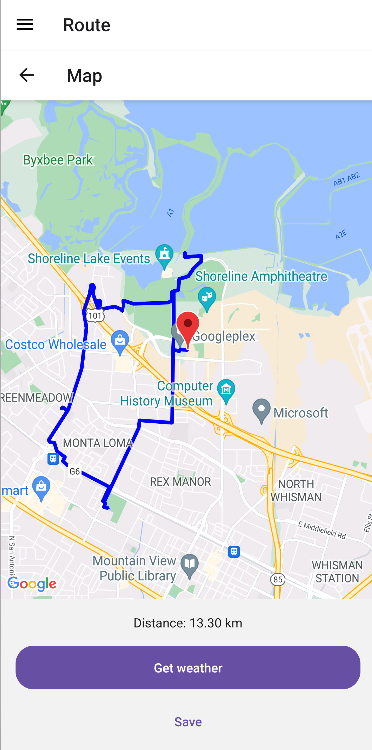
\includegraphics[height=0.5\linewidth]{graphics/10km_route.png}
  \captionof{figure}{He hasn't got shit all over him. The nose? Where'd you get the coconuts? What do you mean? We shall say `Ni' again to you, if you do not appease us}
\end{center}


\section{Conclusies}

De ontwikkeling van de Proof of Concept heeft aangetoond dat het mogelijk is om een eenvoudige maar functionele route-applicatie te bouwen, die gebruikers in staat stelt om routes te plannen en op te slaan met behulp van diverse online tools, zoals Google Maps, OpenStreetMap en OpenWeatherMap.

% \vspace{1cm}


De keuze om de applicatie te ontwikkelen voor het Android-platform biedt een breed bereik, maar er is ook potentieel voor compatibiliteit met iOS-apparaten, hoewel deze mogelijkheid niet uitgebreid is getest. Het gebruik van React Native als ontwikkelingsframework maakt het mogelijk om een native-achtige ervaring te bieden aan gebruikers van verschillende mobiele apparaten.

% \vspace{1cm}


De integratie van een Express.js backend zorgt voor de benodigde connectiviteit met externe tools en services, waardoor de applicatie haar functionaliteit kan uitbreiden en verbeteren. Het testen van de applicatie op zowel fysieke apparaten als emulators draagt bij aan de betrouwbaarheid en prestaties van de applicatie op verschillende platforms.

% \vspace{1cm}


Een belangrijk aspect van de Proof of Concept is de mogelijkheid om de applicatie gratis aan te bieden aan gebruikers, hoewel er mogelijkerwijs extra kosten verbonden zijn aan het toenemende aantal gebruikers. Het bieden van een gratis versie kan de gebruikersacquisitie bevorderen en de adoptie van de applicatie stimuleren.

\section{Toekomstig onderzoek}

In de toekomst kunnen verdere verbeteringen en uitbreidingen worden overwogen, zoals het toevoegen van meer geavanceerde functionaliteiten, verbeterde ondersteuning voor meerdere platforms, en meer integraties met andere platforms die een grote rol spelen in de wereld van loopfanaten. Met voortdurende iteratie en feedback van gebruikers kan de Proof of Concept evolueren tot een volwaardige en veelgebruikte route-applicatie in de markt van mobiele navigatietools.
Concreet zijn er 3 concepten die kunnen worden toegevoegd aan de applicatie. Deze concepten zijn: gebruikerservaring, gegevensverzameling en -presentatie, en algemene optimalisaties. 
\end{multicols}
\end{document}